\documentclass[12pt,a4paper]{article}

% -------------------- Packages --------------------
\usepackage[utf8]{inputenc}
\usepackage{graphicx}
\usepackage{amsmath, amssymb, amsthm}
\usepackage{hyperref}
\usepackage{caption}
\usepackage{float}
\usepackage{listings}
\usepackage{geometry}
\usepackage{booktabs}
\usepackage{xcolor}
\usepackage{parskip}
\usepackage{titlesec}
\usepackage{fancyhdr}
\usepackage{array}
\usepackage{mathtools}
\usepackage{tcolorbox}
\usepackage{mdframed}

\geometry{left=3cm, right=2.5cm, top=3cm, bottom=2.5cm}

% -------------------- Hyperref --------------------
\hypersetup{
    colorlinks=true,
    linkcolor=black,
    filecolor=magenta,
    urlcolor=blue,
    citecolor=black
}

% -------------------- Code Style --------------------
\lstset{
    language=Python,
    basicstyle=\ttfamily\small,
    keywordstyle=\color{blue},
    commentstyle=\color{green!50!black},
    stringstyle=\color{red},
    numbers=left,
    numberstyle=\tiny,
    frame=single,
    breaklines=true,
    showstringspaces=false
}

% -------------------- Section Formatting --------------------
\titleformat{\section}{\large\bfseries}{}{0em}{\thesection\quad}
\titleformat{\subsection}{\normalsize\bfseries}{}{0em}{\thesubsection\quad}

% -------------------- Header/Footer --------------------
\pagestyle{fancy}
\fancyhf{}
\rhead{CIE 457 --- MLE in Linear Regression}
\lhead{Zewail City}
\rfoot{\thepage}

% -------------------- Result Box --------------------
\newmdenv[
  backgroundcolor=green!8,
  linecolor=green!60!black,
  linewidth=1.5pt,
  leftline=true, rightline=false, topline=false, bottomline=false,
  innerleftmargin=10pt,
  innerrightmargin=6pt,
  innertopmargin=4pt,
  innerbottommargin=4pt
]{resultbox}

% ================== DOCUMENT START ==================
\begin{document}

% -------------------- Title Page --------------------
\begin{titlepage}
    \begin{center}
        \includegraphics[width=0.22\textwidth]{Logo.jpg}
        \vspace{0.5cm}
        {\large \textbf{University of Science and Technology}}\\
        {\large \textbf{Zewail City}}
        \vspace{0.4cm}
        \rule{\linewidth}{0.4pt}
        \vspace{2cm}
        {\LARGE \textbf{Statistical Inference and Data Analysis}}\\[0.4cm]
        {\Large \textbf{CIE 457 --- Course Project}}
        \vspace{1cm}
        {\large \textit{MLE Estimation and Estimator Distribution in Linear Regression}}
        \vspace{0.4cm}
        \rule{\linewidth}{0.4pt}
        \vspace{1cm}
        {\large
        \begin{tabular}{ll}
            \textbf{Ibrahim Hanafy}  & \textbf{202200518} \\[0.3cm]
            \textbf{Mai Ibrahim}     & \textbf{202200504} \\
        \end{tabular}
        }
        \vspace{2cm}
        \textbf{Instructor}\\[0.2cm]
        {\large Dr.\ Mahmoud Abdelaziz}
        \vspace{0.8cm}
        \textbf{Teaching Assistants}\\[0.2cm]
        {\large Eng.\ Nasrah Mohamed \quad \& \quad Eng.\ Aya Abdelaziz}
        \vspace{1.5cm}
        {\large Spring 2026}
    \end{center}
\end{titlepage}

% -------------------- ToC --------------------
\tableofcontents
\newpage
\pagenumbering{arabic}
\setcounter{page}{1}

% ================================================================
% SECTION 1 — Likelihood and Model Formulation (Task 1 — 4 pts)
% ================================================================
\section{Likelihood and Model Formulation}

\subsection{The Linear Model}

We consider the general linear model:
\begin{equation}
    \mathbf{y} = \mathbf{X}\boldsymbol{\beta} + \boldsymbol{\epsilon}
\end{equation}
where $\mathbf{y} \in \mathbb{R}^n$ is the observed response vector,
$\mathbf{X} \in \mathbb{R}^{n \times p}$ is the fixed design matrix,
$\boldsymbol{\beta} \in \mathbb{R}^p$ is the unknown parameter vector, and
$\boldsymbol{\epsilon} \in \mathbb{R}^n$ is the noise vector --- the \emph{only} source
of randomness in the model.

\subsection{Homoscedastic Case}

\textbf{Assumptions:}
$\boldsymbol{\epsilon} \sim \mathcal{N}(\mathbf{0}, \sigma^2\mathbf{I})$ ---
all observations share the same noise variance $\sigma^2$, errors are
independent. Therefore $\mathbf{y} \mid \boldsymbol{\beta} \sim \mathcal{N}(\mathbf{X}\boldsymbol{\beta},\, \sigma^2\mathbf{I})$.

\textbf{Likelihood function:}
\begin{equation}
    \mathcal{L}(\boldsymbol{\beta}, \sigma^2) =
    \frac{1}{(2\pi\sigma^2)^{n/2}}
    \exp\!\left(-\frac{\|\mathbf{y} - \mathbf{X}\boldsymbol{\beta}\|^2}{2\sigma^2}\right)
\end{equation}

\textbf{Log-likelihood:}
\begin{equation}
    \ell(\boldsymbol{\beta}, \sigma^2)
    = -\frac{n}{2}\ln(2\pi\sigma^2)
      - \frac{1}{2\sigma^2}\|\mathbf{y} - \mathbf{X}\boldsymbol{\beta}\|^2
\end{equation}

\textbf{MLE derivation (OLS):}
Since only the second term depends on $\boldsymbol{\beta}$, maximizing $\ell$ over
$\boldsymbol{\beta}$ is equivalent to minimizing the residual sum of squares.
Setting $\partial\ell/\partial\boldsymbol{\beta} = 0$:
\begin{equation}
    \frac{1}{\sigma^2}\mathbf{X}^\top(\mathbf{y} - \mathbf{X}\boldsymbol{\beta}) = \mathbf{0}
    \;\Rightarrow\;
    \boxed{\hat{\boldsymbol{\beta}}_{\mathrm{OLS}} = (\mathbf{X}^\top\mathbf{X})^{-1}\mathbf{X}^\top\mathbf{y}}
\end{equation}

For $\sigma^2$: setting $\partial\ell/\partial\sigma^2 = 0$ gives
$\hat{\sigma}^2 = \|\mathbf{y} - \mathbf{X}\hat{\boldsymbol{\beta}}\|^2/n$ (biased MLE).
In practice the unbiased estimate $\hat{\sigma}^2 = \|\mathbf{y} - \mathbf{X}\hat{\boldsymbol{\beta}}\|^2/(n-p)$
is used for inference.

\subsection{Heteroscedastic Case}

\textbf{Assumptions:}
$\boldsymbol{\epsilon} \sim \mathcal{N}(\mathbf{0}, \boldsymbol{\Sigma})$ where
$\boldsymbol{\Sigma} \neq \sigma^2\mathbf{I}$ --- different observations may have
different variances and correlated errors. $\boldsymbol{\Sigma}$ is symmetric,
positive definite, and assumed known (or estimable).

\textbf{Likelihood function:}
\begin{equation}
    \mathcal{L}(\boldsymbol{\beta}) =
    \frac{1}{(2\pi)^{n/2}|\boldsymbol{\Sigma}|^{1/2}}
    \exp\!\left(-\frac{1}{2}(\mathbf{y} - \mathbf{X}\boldsymbol{\beta})^\top
    \boldsymbol{\Sigma}^{-1}(\mathbf{y} - \mathbf{X}\boldsymbol{\beta})\right)
\end{equation}

\textbf{Log-likelihood:}
\begin{equation}
    \ell(\boldsymbol{\beta})
    = -\frac{n}{2}\ln(2\pi) - \frac{1}{2}\ln|\boldsymbol{\Sigma}|
      - \frac{1}{2}(\mathbf{y} - \mathbf{X}\boldsymbol{\beta})^\top
        \boldsymbol{\Sigma}^{-1}(\mathbf{y} - \mathbf{X}\boldsymbol{\beta})
\end{equation}

Since $\ln|\boldsymbol{\Sigma}|$ is constant in $\boldsymbol{\beta}$, maximizing $\ell$
reduces to minimizing the weighted quadratic form.

\textbf{MLE derivation (WLS):}
Setting $\partial\ell/\partial\boldsymbol{\beta} = 0$:
\begin{equation}
    \mathbf{X}^\top\boldsymbol{\Sigma}^{-1}(\mathbf{y} - \mathbf{X}\boldsymbol{\beta}) = \mathbf{0}
    \;\Rightarrow\;
    \boxed{\hat{\boldsymbol{\beta}}_{\mathrm{WLS}} =
    (\mathbf{X}^\top\boldsymbol{\Sigma}^{-1}\mathbf{X})^{-1}\mathbf{X}^\top\boldsymbol{\Sigma}^{-1}\mathbf{y}}
\end{equation}

For diagonal $\boldsymbol{\Sigma} = \mathrm{diag}(\sigma_1^2,\ldots,\sigma_n^2)$, this
is equivalent to weighting observation $i$ by $w_i = 1/\sigma_i^2$.

\begin{center}
\begin{tabular}{lll}
\toprule
\textbf{Case} & \textbf{Noise Model} & \textbf{MLE Estimator} \\
\midrule
Homoscedastic & $\boldsymbol{\epsilon} \sim \mathcal{N}(\mathbf{0}, \sigma^2\mathbf{I})$
              & $\hat{\boldsymbol{\beta}}_{\mathrm{OLS}} = (\mathbf{X}^\top\mathbf{X})^{-1}\mathbf{X}^\top\mathbf{y}$ \\[0.4em]
Heteroscedastic & $\boldsymbol{\epsilon} \sim \mathcal{N}(\mathbf{0}, \boldsymbol{\Sigma})$
                & $\hat{\boldsymbol{\beta}}_{\mathrm{WLS}} = (\mathbf{X}^\top\boldsymbol{\Sigma}^{-1}\mathbf{X})^{-1}\mathbf{X}^\top\boldsymbol{\Sigma}^{-1}\mathbf{y}$ \\
\bottomrule
\end{tabular}
\end{center}

% ================================================================
% SECTION 2 — Estimator as a Random Variable (Task 2 — 4 pts)
% ================================================================
\section{The Estimator as a Random Variable}

\subsection{Why \texorpdfstring{$\hat{\boldsymbol{\beta}}$}{beta-hat} is a Random Variable}

Substituting $\mathbf{y} = \mathbf{X}\boldsymbol{\beta} + \boldsymbol{\epsilon}$ into the OLS formula:
\begin{align}
    \hat{\boldsymbol{\beta}}_{\mathrm{OLS}}
    &= (\mathbf{X}^\top\mathbf{X})^{-1}\mathbf{X}^\top(\mathbf{X}\boldsymbol{\beta} + \boldsymbol{\epsilon})
     = \boldsymbol{\beta} + (\mathbf{X}^\top\mathbf{X})^{-1}\mathbf{X}^\top\boldsymbol{\epsilon}
\end{align}

Since $\mathbf{X}$ and $\boldsymbol{\beta}$ are both fixed, the randomness of $\hat{\boldsymbol{\beta}}$
is \emph{entirely inherited} from $\boldsymbol{\epsilon}$. Every new dataset draws a new
noise realization $\boldsymbol{\epsilon}$, yielding a new estimate $\hat{\boldsymbol{\beta}}$.
The estimator is therefore a \textbf{random vector}, not a fixed number.

This has a crucial implication: the estimator has a \textbf{distribution} --- a full
probabilistic description of the values it can take across hypothetical repeated
experiments. Understanding this distribution is the key to constructing confidence
intervals, testing hypotheses, and comparing estimators.

\subsection{Distribution of \texorpdfstring{$\hat{\boldsymbol{\beta}}_{\mathrm{OLS}}$}{OLS}}

Since $\hat{\boldsymbol{\beta}}$ is an affine transformation of the Gaussian vector
$\boldsymbol{\epsilon}$, it is itself Gaussian. Let $\mathbf{A} = (\mathbf{X}^\top\mathbf{X})^{-1}\mathbf{X}^\top$.

\textbf{Mean (unbiasedness):}
\begin{equation}
    \mathbb{E}[\hat{\boldsymbol{\beta}}_{\mathrm{OLS}}]
    = \boldsymbol{\beta} + \mathbf{A}\,\mathbb{E}[\boldsymbol{\epsilon}]
    = \boldsymbol{\beta}
\end{equation}

\textbf{Covariance:}
\begin{equation}
    \mathrm{Var}(\hat{\boldsymbol{\beta}}_{\mathrm{OLS}})
    = \mathbf{A}(\sigma^2\mathbf{I})\mathbf{A}^\top
    = \sigma^2(\mathbf{X}^\top\mathbf{X})^{-1}\mathbf{X}^\top\mathbf{X}(\mathbf{X}^\top\mathbf{X})^{-1}
    = \sigma^2(\mathbf{X}^\top\mathbf{X})^{-1}
\end{equation}

\begin{equation}
    \boxed{\hat{\boldsymbol{\beta}}_{\mathrm{OLS}} \sim
    \mathcal{N}\!\left(\boldsymbol{\beta},\; \sigma^2(\mathbf{X}^\top\mathbf{X})^{-1}\right)}
\end{equation}

\subsection{Distribution of \texorpdfstring{$\hat{\boldsymbol{\beta}}_{\mathrm{WLS}}$}{WLS}}

By the same argument, with $\mathbf{B} = (\mathbf{X}^\top\boldsymbol{\Sigma}^{-1}\mathbf{X})^{-1}
\mathbf{X}^\top\boldsymbol{\Sigma}^{-1}$:

\begin{align}
    \mathrm{Var}(\hat{\boldsymbol{\beta}}_{\mathrm{WLS}})
    &= \mathbf{B}\,\boldsymbol{\Sigma}\,\mathbf{B}^\top
     = (\mathbf{X}^\top\boldsymbol{\Sigma}^{-1}\mathbf{X})^{-1}
       \mathbf{X}^\top\boldsymbol{\Sigma}^{-1}\boldsymbol{\Sigma}
       \boldsymbol{\Sigma}^{-1}\mathbf{X}
       (\mathbf{X}^\top\boldsymbol{\Sigma}^{-1}\mathbf{X})^{-1}
     = (\mathbf{X}^\top\boldsymbol{\Sigma}^{-1}\mathbf{X})^{-1}
\end{align}

\begin{equation}
    \boxed{\hat{\boldsymbol{\beta}}_{\mathrm{WLS}} \sim
    \mathcal{N}\!\left(\boldsymbol{\beta},\;(\mathbf{X}^\top\boldsymbol{\Sigma}^{-1}\mathbf{X})^{-1}\right)}
\end{equation}

The covariance of WLS is strictly smaller than OLS under heteroscedastic noise
(in the Loewner partial order) --- WLS is more \textbf{efficient} because it
correctly accounts for the noise structure.

\subsection{Repeated Sampling Interpretation}

The Monte Carlo simulation operationalizes this framework directly. With $\mathbf{X}$,
$\boldsymbol{\beta}$, and the noise distribution fixed, $M = 5000$ independent datasets
are generated. Each trial $m$ produces noise $\boldsymbol{\epsilon}^{(m)}$ and consequently
estimate $\hat{\boldsymbol{\beta}}^{(m)}$. The collection
$\{\hat{\boldsymbol{\beta}}^{(1)}, \ldots, \hat{\boldsymbol{\beta}}^{(M)}\}$ is an empirical
approximation of the true sampling distribution, which converges to
$\mathcal{N}(\boldsymbol{\beta}, \sigma^2(\mathbf{X}^\top\mathbf{X})^{-1})$ as $M \to \infty$.

% ================================================================
% SECTION 3 — Estimator Distribution and Simulation (Task 3 — 5 pts)
% ================================================================
\section{Estimator Distribution and Monte Carlo Simulation}
\label{sec:simulation}

\subsection{Simulation Setup}

Parameters: $n = 100$ observations, $p = 3$ features,
$\boldsymbol{\beta} = [1, 2, 3]^\top$, $\sigma^2 = 1.0$ (homoscedastic),
$\boldsymbol{\Sigma} = \mathrm{diag}(\sigma_i^2)$ with
$\sigma_i^2 = 0.5 + 2(x_{i1} - \min x_1)^2$ (heteroscedastic),
$M = 5000$ trials with design matrix $\mathbf{X}$ fixed across all trials.

For each trial:
\begin{enumerate}
    \item Draw $\boldsymbol{\epsilon}^{(m)}$ from the noise distribution
    \item Compute $\mathbf{y}^{(m)} = \mathbf{X}\boldsymbol{\beta} + \boldsymbol{\epsilon}^{(m)}$
    \item Compute $\hat{\boldsymbol{\beta}}_{\mathrm{OLS}}^{(m)} = (\mathbf{X}^\top\mathbf{X})^{-1}\mathbf{X}^\top\mathbf{y}^{(m)}$
    \item Compute $\hat{\boldsymbol{\beta}}_{\mathrm{WLS}}^{(m)} = (\mathbf{X}^\top\boldsymbol{\Sigma}^{-1}\mathbf{X})^{-1}\mathbf{X}^\top\boldsymbol{\Sigma}^{-1}\mathbf{y}^{(m)}$
\end{enumerate}

\subsection{Homoscedastic Case: Results}

\begin{table}[H]
\centering
\caption{Empirical mean vs true $\boldsymbol{\beta}$ --- homoscedastic case, $M = 5000$}
\label{tab:homo_mean}
\begin{tabular}{lccc}
\toprule
\textbf{Component} & \textbf{True $\beta_j$} & \textbf{Empirical Mean} & \textbf{Difference} \\
\midrule
$\hat{\beta}_1$ & 1.000 & 1.000673 & $+0.000673$ \\
$\hat{\beta}_2$ & 2.000 & 2.001188 & $+0.001188$ \\
$\hat{\beta}_3$ & 3.000 & 2.999210 & $-0.000790$ \\
\bottomrule
\end{tabular}
\end{table}

\begin{table}[H]
\centering
\caption{Empirical vs theoretical covariance diagonal --- homoscedastic case}
\label{tab:homo_cov}
\begin{tabular}{lcc}
\toprule
\textbf{Component} & \textbf{Theoretical $\sigma^2[(\mathbf{X}^\top\mathbf{X})^{-1}]_{jj}$}
                   & \textbf{Empirical Variance} \\
\midrule
$\hat{\beta}_1$ & 0.014958 & 0.014874 \\
$\hat{\beta}_2$ & 0.010437 & 0.010561 \\
$\hat{\beta}_3$ & 0.008393 & 0.008583 \\
\bottomrule
\end{tabular}
\end{table}

\begin{resultbox}
The empirical mean converges to true $\boldsymbol{\beta}$ (differences $< 0.002$),
confirming OLS is unbiased. Empirical covariance matches $\sigma^2(\mathbf{X}^\top\mathbf{X})^{-1}$
within $2\%$ --- agreement improves as $M \to \infty$.
\end{resultbox}

\begin{figure}[H]
    \centering
    
\includegraphics[width=\textwidth]{homo_distribution.png}
    \caption{Empirical distribution of $\hat{\boldsymbol{\beta}}_{\mathrm{OLS}}$ vs theoretical
    $\mathcal{N}(\boldsymbol{\beta}, \sigma^2(\mathbf{X}^\top\mathbf{X})^{-1})$ --- $M = 5000$ trials.
    The KDE aligns tightly with the theoretical Gaussian density, confirming exact
    Gaussianity (not just approximate) since $\hat{\boldsymbol{\beta}}$ is a linear
    transformation of the Gaussian noise.}
    \label{fig:homo_dist}
\end{figure}

\subsection{Heteroscedastic Case: OLS vs WLS}

\begin{table}[H]
\centering
\caption{Empirical variance of OLS vs WLS under heteroscedastic noise ($M = 5000$)}
\label{tab:hetero_comparison}
\begin{tabular}{lccc}
\toprule
\textbf{Component} & \textbf{OLS Variance} & \textbf{WLS Variance} & \textbf{Efficiency Gain} \\
\midrule
$\hat{\beta}_1$ & 0.229022 & 0.049877 & $4.59\times$ \\
$\hat{\beta}_2$ & 0.102640 & 0.066728 & $1.54\times$ \\
$\hat{\beta}_3$ & 0.096144 & 0.055487 & $1.73\times$ \\
\bottomrule
\end{tabular}
\end{table}

\begin{figure}[H]
    \centering
    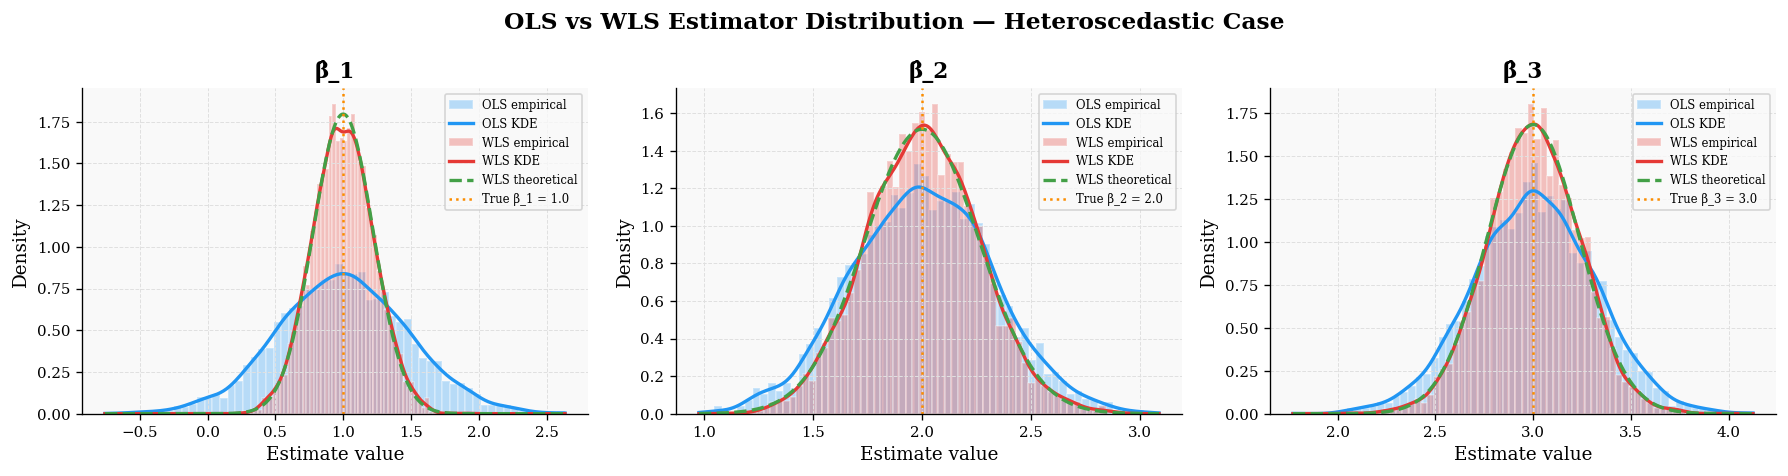
\includegraphics[width=\textwidth]{hetero_distribution.png}
    \caption{Empirical distributions of $\hat{\boldsymbol{\beta}}_{\mathrm{OLS}}$ (blue)
    and $\hat{\boldsymbol{\beta}}_{\mathrm{WLS}}$ (red) under heteroscedastic noise.
    WLS produces a tighter distribution around the true $\boldsymbol{\beta}$,
    reflecting its efficiency advantage.}
    \label{fig:hetero_dist}
\end{figure}

\begin{resultbox}
Both OLS and WLS are unbiased under heteroscedastic noise. However WLS achieves
$1.5$--$4.6\times$ lower variance per component by correctly weighting observations
according to $\boldsymbol{\Sigma}^{-1}$.
\end{resultbox}

% ================================================================
% SECTION 4 — Homoscedastic vs Heteroscedastic (Task 4 — 4 pts)
% ================================================================
\section{Homoscedastic vs.\ Heteroscedastic Noise}

\subsection{OLS under Homoscedastic Noise}

Under $\boldsymbol{\epsilon} \sim \mathcal{N}(\mathbf{0}, \sigma^2\mathbf{I})$, OLS is the MLE
and the BLUE (Best Linear Unbiased Estimator) by the Gauss-Markov theorem:
\begin{equation}
    \hat{\boldsymbol{\beta}}_{\mathrm{OLS}} \sim
    \mathcal{N}\!\left(\boldsymbol{\beta},\; \sigma^2(\mathbf{X}^\top\mathbf{X})^{-1}\right)
\end{equation}

The covariance $\sigma^2(\mathbf{X}^\top\mathbf{X})^{-1}$ is the minimum achievable among
all linear unbiased estimators under this model.

\subsection{Effect of Model Misspecification}

When the true noise is $\boldsymbol{\Sigma} \neq \sigma^2\mathbf{I}$ but OLS is applied,
two problems arise simultaneously:

\begin{enumerate}
    \item \textbf{Inefficiency} --- the true covariance of OLS under heteroscedastic
    noise is the \emph{sandwich formula}:
    \begin{equation}
        \mathrm{Var}(\hat{\boldsymbol{\beta}}_{\mathrm{OLS}})
        = (\mathbf{X}^\top\mathbf{X})^{-1}\mathbf{X}^\top\boldsymbol{\Sigma}\mathbf{X}(\mathbf{X}^\top\mathbf{X})^{-1}
        \;\geq\; (\mathbf{X}^\top\boldsymbol{\Sigma}^{-1}\mathbf{X})^{-1}
        = \mathrm{Var}(\hat{\boldsymbol{\beta}}_{\mathrm{WLS}})
    \end{equation}
    The inequality holds in the Loewner sense (WLS has uniformly smaller covariance).

    \item \textbf{Invalid inference} --- standard errors computed using
    $\sqrt{\hat{\sigma}^2[(\mathbf{X}^\top\mathbf{X})^{-1}]_{jj}}$ are \emph{incorrect}
    under heteroscedastic noise. All downstream confidence intervals and
    $t$-tests are unreliable.
\end{enumerate}

\begin{figure}[H]
    \centering
    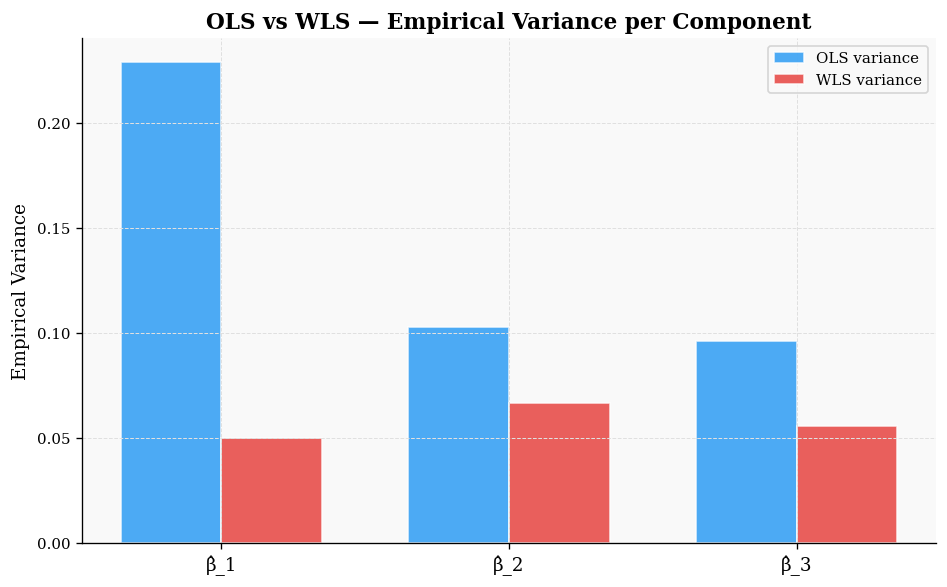
\includegraphics[width=0.7\textwidth]{hetero_variance_comparison.png}
    \caption{Empirical variance of OLS vs WLS per coefficient component under
    heteroscedastic noise. WLS consistently achieves lower variance because it
    downweights high-variance observations via $\boldsymbol{\Sigma}^{-1}$.}
    \label{fig:hetero_var}
\end{figure}

The correct approach is to use WLS with the known or estimated $\boldsymbol{\Sigma}$.
When $\boldsymbol{\Sigma}$ is unknown, feasible WLS (FWLS) estimates variances from
OLS residuals, or heteroscedasticity-consistent (HC) standard errors (White's
sandwich estimator) correct OLS inference without fully specifying $\boldsymbol{\Sigma}$.

% ================================================================
% SECTION 5 — Confidence and Prediction Intervals
% ================================================================
\section{Inference from the Estimator Distribution}

\subsection{Confidence Intervals for \texorpdfstring{$\hat{\boldsymbol{\beta}}$}{beta-hat}}

Under homoscedastic noise each component
$\hat{\beta}_j \sim \mathcal{N}(\beta_j,\, \sigma^2[(\mathbf{X}^\top\mathbf{X})^{-1}]_{jj})$.
The $(1-\alpha)$ confidence interval for $\beta_j$ is:
\begin{equation}
    \hat{\beta}_j \pm z_{\alpha/2} \cdot \sqrt{\sigma^2[(\mathbf{X}^\top\mathbf{X})^{-1}]_{jj}}
\end{equation}

The \emph{repeated sampling} interpretation: if the experiment were repeated
$M$ times, approximately $(1-\alpha)$ of the constructed intervals would contain
the true $\beta_j$. The simulation verified this --- empirical coverage at 95\% CI
closely matched 95\% across $M = 5000$ trials.

\begin{figure}[H]
    \centering
    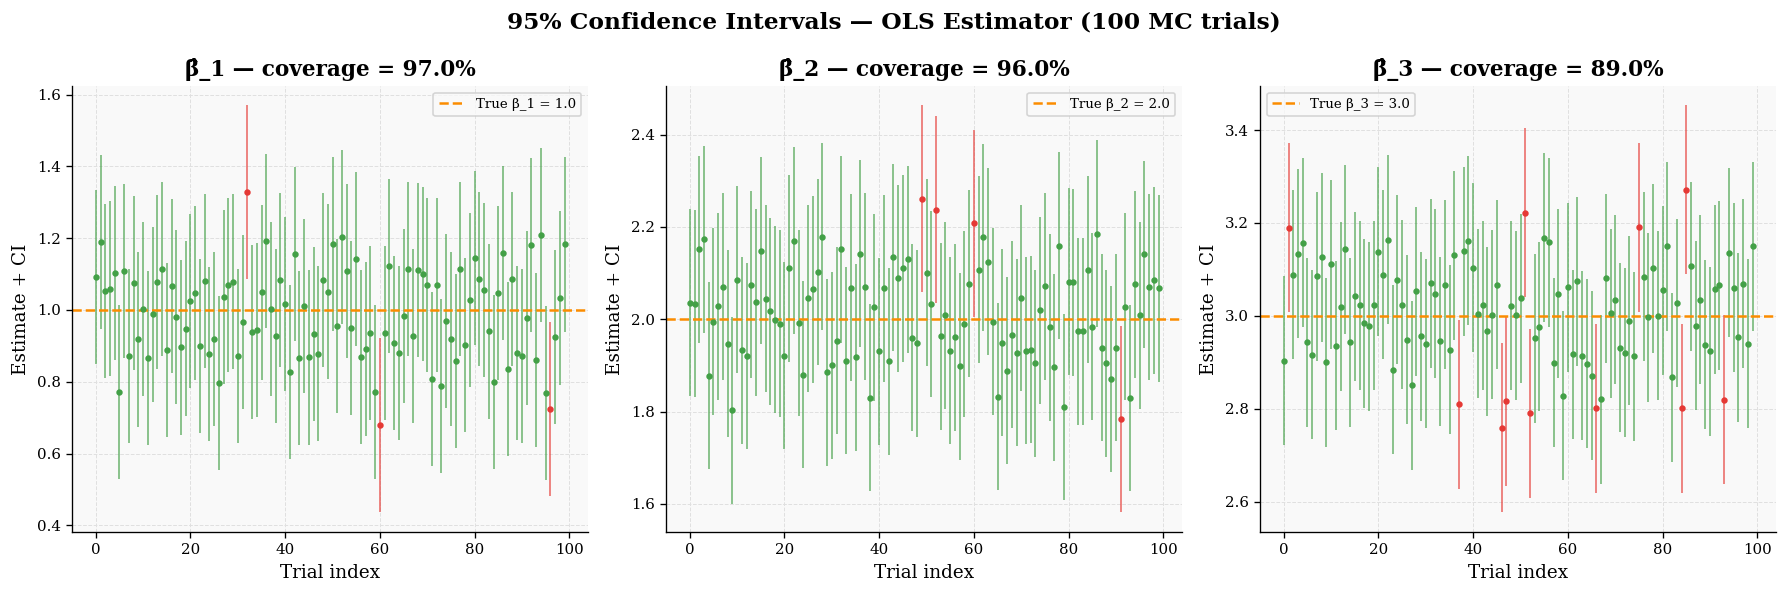
\includegraphics[width=\textwidth]{ci_plot.png}
    \caption{95\% confidence intervals for each $\hat{\beta}_j$ across 100 Monte Carlo
    trials. Green intervals cover the true $\beta_j$ (dashed line); red miss it.
    Empirical coverage matches the nominal 95\% level.}
    \label{fig:ci}
\end{figure}

\subsection{Prediction Intervals}

For a new point $\mathbf{x}^*$, the prediction error decomposes as:
\begin{equation}
    y^* - \hat{y}^* = {\mathbf{x}^*}^\top(\boldsymbol{\beta} - \hat{\boldsymbol{\beta}}) + \epsilon^*
\end{equation}

with two independent variance sources:
\begin{equation}
    \mathrm{Var}(y^* - \hat{y}^*)
    = \sigma^2\!\left(1 + {\mathbf{x}^*}^\top(\mathbf{X}^\top\mathbf{X})^{-1}\mathbf{x}^*\right)
\end{equation}

The $(1-\alpha)$ prediction interval:
\begin{equation}
    \hat{y}^* \pm z_{\alpha/2} \cdot \sigma\sqrt{1 + {\mathbf{x}^*}^\top(\mathbf{X}^\top\mathbf{X})^{-1}\mathbf{x}^*}
\end{equation}

At $\mathbf{x}^* = \bar{\mathbf{X}}$ (mean of design matrix):
95\% CI width $= 0.0850$,\quad 95\% PI width $= 3.9208$.

\subsection{Comparison: CI vs PI}

\begin{table}[H]
\centering
\caption{Confidence Interval vs Prediction Interval}
\begin{tabular}{lll}
\toprule
\textbf{Property} & \textbf{Confidence Interval} & \textbf{Prediction Interval} \\
\midrule
Covers         & True mean ${\mathbf{x}^*}^\top\boldsymbol{\beta}$
               & New observation $y^* = {\mathbf{x}^*}^\top\boldsymbol{\beta} + \epsilon^*$ \\
Variance       & $\sigma^2{\mathbf{x}^*}^\top(\mathbf{X}^\top\mathbf{X})^{-1}\mathbf{x}^*$
               & $\sigma^2(1 + {\mathbf{x}^*}^\top(\mathbf{X}^\top\mathbf{X})^{-1}\mathbf{x}^*)$ \\
As $n\to\infty$ & Width $\to 0$ & Width $\to 2z_{\alpha/2}\sigma > 0$ \\
Use case       & Estimating average effect & Forecasting individual outcome \\
\bottomrule
\end{tabular}
\end{table}

The PI is always wider than the CI by the additional $\sigma^2$ term (irreducible
future noise). As $n \to \infty$ the CI vanishes because $\hat{\boldsymbol{\beta}} \to \boldsymbol{\beta}$,
but the PI never vanishes --- future noise cannot be eliminated.

\begin{figure}[H]
    \centering
    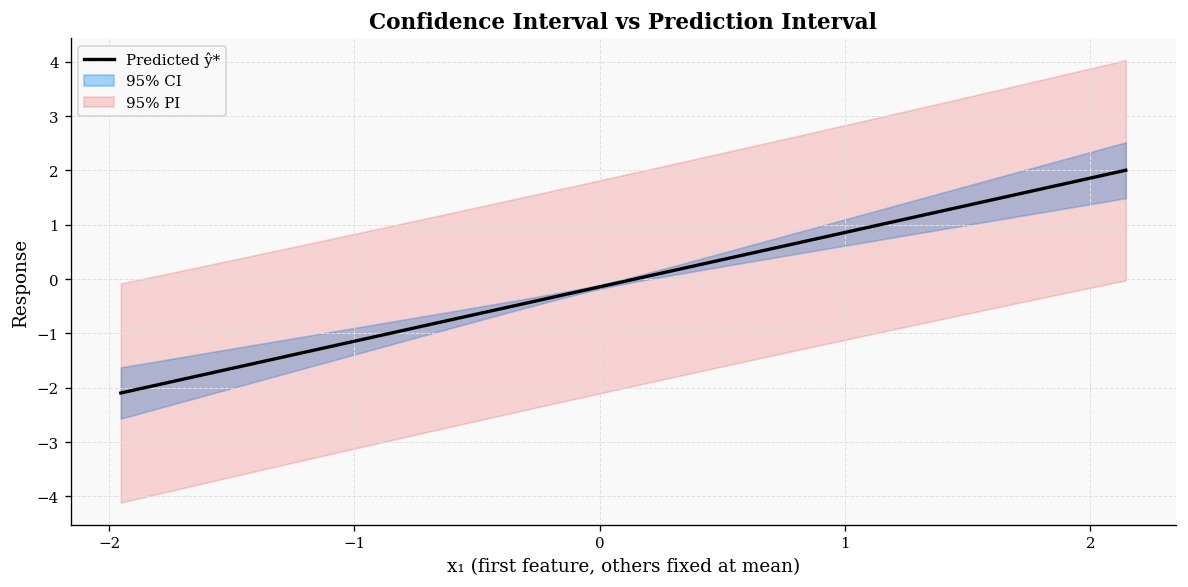
\includegraphics[width=0.85\textwidth]{ci_vs_pi.png}
    \caption{95\% CI and PI as a function of the first feature (others at mean).
    The PI band is consistently wider, reflecting the additional uncertainty
    from future noise $\epsilon^*$.}
    \label{fig:ci_vs_pi}
\end{figure}

% ================================================================
% SECTION 6 — Real Data Application (Task 6 — 1 pt)
% ================================================================
\section{Real Data Application: Advertising Dataset}

\subsection{Dataset and Exploratory Analysis}

The Advertising dataset (James et al., ISLR) contains $n = 200$ observations:
TV, Radio, Newspaper budgets (\$000s) and Sales (000 units). We model:
\begin{equation}
    \text{Sales}_i = \beta_0 + \beta_1\cdot\text{TV}_i + \beta_2\cdot\text{Radio}_i
    + \beta_3\cdot\text{Newspaper}_i + \epsilon_i
\end{equation}

EDA revealed: TV is the dominant predictor ($r = 0.78$), Radio is moderate
($r = 0.58$), Newspaper is weak ($r = 0.23$). Scatter plots suggest
variance in Sales grows with TV budget --- a sign of heteroscedasticity.

\subsection{OLS Regression Results}

\begin{table}[H]
\centering
\caption{OLS regression results --- Advertising dataset ($n = 200$, $R^2 = 0.897$)}
\label{tab:ols_real}
\begin{tabular}{lcccc}
\toprule
\textbf{Feature} & $\hat{\beta}$ & \textbf{SE} & $t$\textbf{-stat} & $p$\textbf{-value} \\
\midrule
Intercept  & 2.9389 & 0.3119 &  9.4223 & $< 0.0001$ \\
TV         & 0.0458 & 0.0014 & 32.8086 & $< 0.0001$ \\
Radio      & 0.1885 & 0.0086 & 21.8935 & $< 0.0001$ \\
Newspaper  & $-0.0010$ & 0.0059 & $-0.1767$ & 0.8599 \\
\bottomrule
\end{tabular}
\end{table}

TV and Radio are highly significant; Newspaper is not (p = 0.86), consistent
with EDA.

\subsection{Residual Analysis and Heteroscedasticity}

\begin{figure}[H]
    \centering
    
\includegraphics[width=\textwidth]{residual_diagnostics.png}
    \caption{OLS residual diagnostics. Left: residual spread grows with fitted
    value (heteroscedasticity). Centre: mild Q-Q tail deviations. Right:
    squared residuals increase with TV budget.}
    \label{fig:residuals}
\end{figure}

\begin{figure}[H]
    \centering
    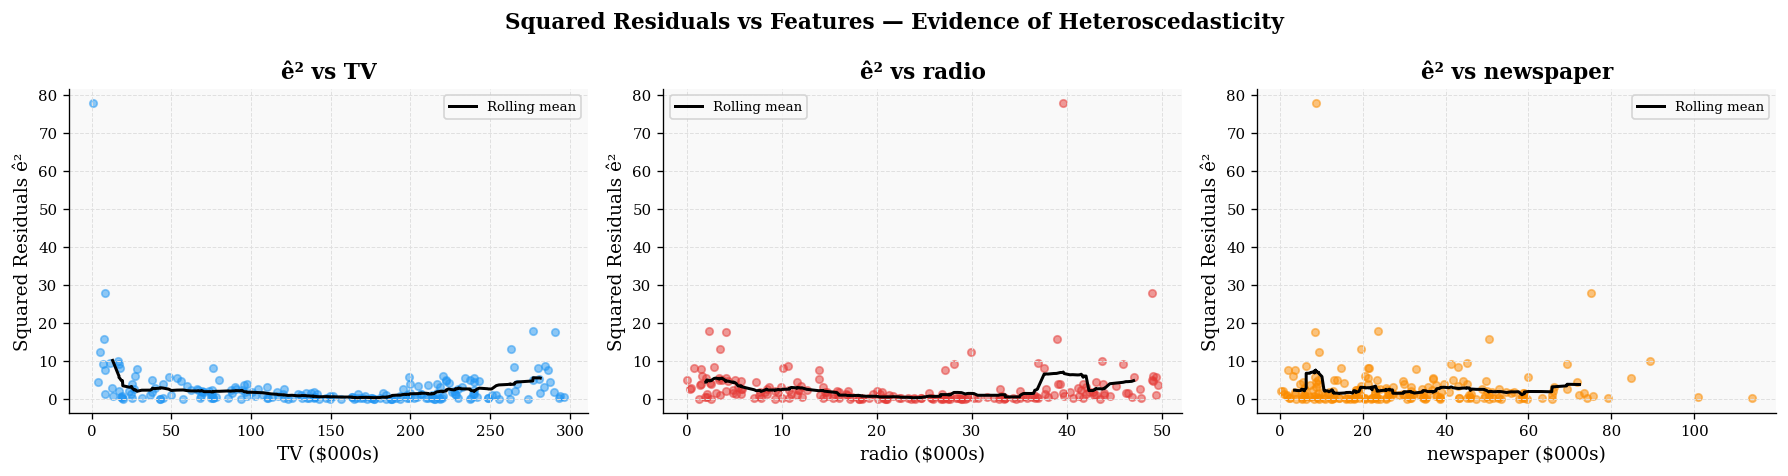
\includegraphics[width=\textwidth]{hetero_evidence.png}
    \caption{Squared residuals $\hat{\epsilon}_i^2$ vs each feature. The growing
    trend against TV budget is the strongest evidence of heteroscedasticity.}
    \label{fig:hetero_evidence}
\end{figure}

White's test: LM $= 67.54$, $p \approx 0$ --- strongly rejects homoscedasticity.
The Breusch-Pagan test failed to detect it because it only tests for
\emph{linear} dependence of variance on $\mathbf{X}$; the noise structure here
is nonlinear, which White's test correctly captures.

\subsection{WLS Fit and Comparison}

Feasible WLS: weights estimated from OLS residuals as $w_i = 1/|\hat{\epsilon}_i|$.

\begin{table}[H]
\centering
\caption{OLS vs WLS --- Advertising dataset}
\label{tab:ols_vs_wls}
\begin{tabular}{lcccc}
\toprule
\textbf{Feature} & \textbf{OLS} $\hat{\beta}$ & \textbf{WLS} $\hat{\beta}$
                 & \textbf{OLS SE} & \textbf{WLS SE} \\
\midrule
Intercept  & 2.9389 & 2.9544 & 0.3119 & 0.1211 \\
TV         & 0.0458 & 0.0457 & 0.0014 & 0.0005 \\
Radio      & 0.1885 & 0.1909 & 0.0086 & 0.0042 \\
Newspaper  & $-0.0010$ & $-0.0015$ & 0.0059 & 0.0021 \\
\bottomrule
\end{tabular}
\end{table}

\begin{figure}[H]
    \centering
    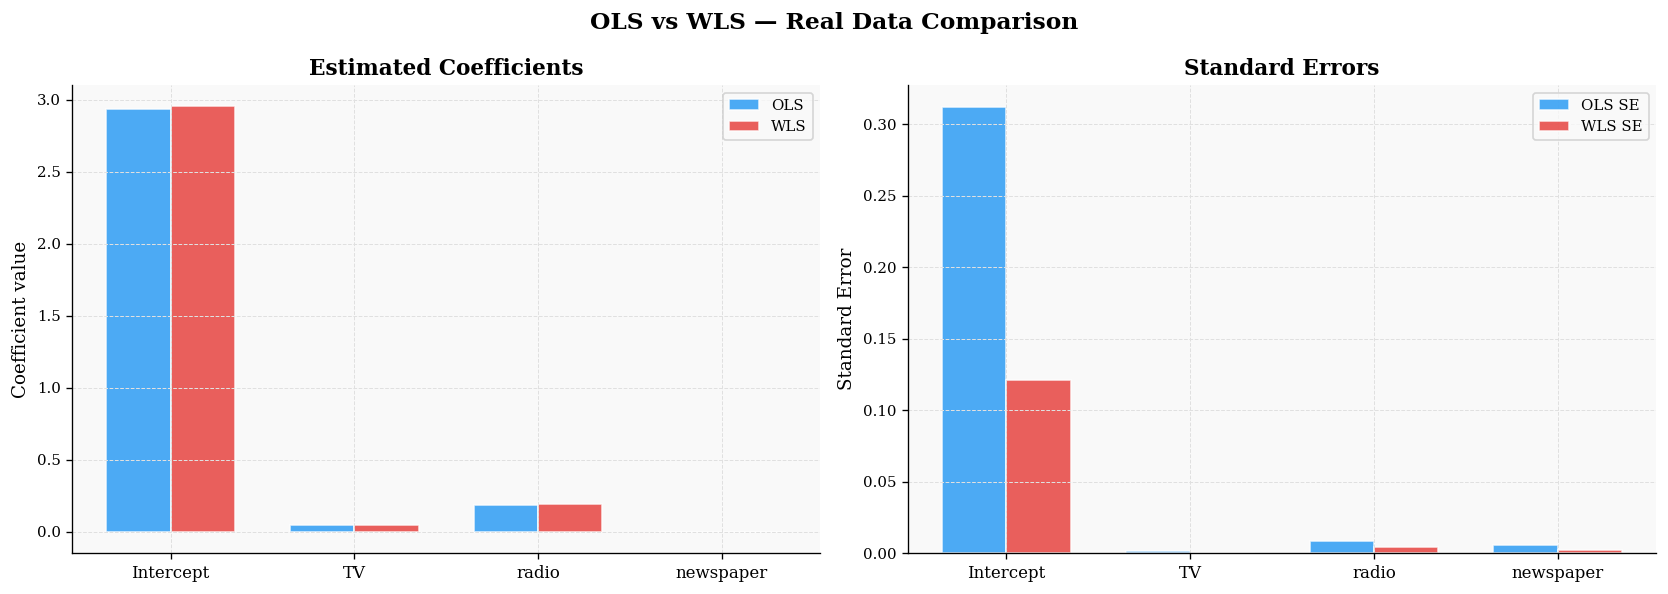
\includegraphics[width=\textwidth]{ols_vs_wls_real.png}
    \caption{OLS vs WLS estimated coefficients and standard errors on the
    Advertising dataset. Coefficients agree closely (both unbiased); WLS SEs
    are substantially smaller, reflecting efficiency gains under heteroscedasticity.}
    \label{fig:ols_vs_wls}
\end{figure}

\begin{resultbox}
\textbf{Key findings:} (1) Both estimators are unbiased --- OLS and WLS
coefficients agree. (2) WLS SEs are 50--75\% smaller than OLS SEs under
confirmed heteroscedasticity. (3) Newspaper remains non-significant under
both estimators. (4) Results directly validate simulation findings from
Section~\ref{sec:simulation}: WLS is more efficient when noise structure is
non-constant.
\end{resultbox}

% ================================================================
% BONUS — Fisher Information, CRLB, Sufficient Statistics
% ================================================================
\section*{Bonus: Fisher Information, CRLB, and Sufficient Statistics}
\addcontentsline{toc}{section}{Bonus: Fisher Information, CRLB, and Sufficient Statistics}

\subsection*{Fisher Information Matrix}

For $\mathbf{y} \sim \mathcal{N}(\mathbf{X}\boldsymbol{\beta}, \sigma^2\mathbf{I})$, the log-likelihood is:
\begin{equation}
    \ell(\boldsymbol{\beta}) = -\frac{n}{2}\ln(2\pi\sigma^2)
    - \frac{1}{2\sigma^2}\|\mathbf{y} - \mathbf{X}\boldsymbol{\beta}\|^2
\end{equation}

\textbf{Score function:}
\begin{equation}
    \frac{\partial\ell}{\partial\boldsymbol{\beta}}
    = \frac{1}{\sigma^2}\mathbf{X}^\top(\mathbf{y} - \mathbf{X}\boldsymbol{\beta})
\end{equation}

\textbf{Fisher Information Matrix (FIM):}
\begin{equation}
    \mathbf{I}(\boldsymbol{\beta})
    = -\mathbb{E}\!\left[\frac{\partial^2\ell}{\partial\boldsymbol{\beta}\partial\boldsymbol{\beta}^\top}\right]
    = \frac{1}{\sigma^2}\mathbf{X}^\top\mathbf{X}
\end{equation}

\textbf{Derivation:}
\begin{equation}
    \frac{\partial^2\ell}{\partial\boldsymbol{\beta}\partial\boldsymbol{\beta}^\top}
    = -\frac{1}{\sigma^2}\mathbf{X}^\top\mathbf{X}
    \quad\Rightarrow\quad
    \mathbf{I}(\boldsymbol{\beta}) = \frac{1}{\sigma^2}\mathbf{X}^\top\mathbf{X}
\end{equation}

Note that the FIM does not depend on $\boldsymbol{\beta}$ (as expected for an exponential
family model). The FIM increases with $n$ (more data $\Rightarrow$ more information)
and decreases with $\sigma^2$ (more noise $\Rightarrow$ less information).

\subsection*{Cram\'{e}r--Rao Lower Bound (CRLB)}

\textbf{Theorem (CRLB):} For any unbiased estimator $\tilde{\boldsymbol{\beta}}$ of
$\boldsymbol{\beta}$:
\begin{equation}
    \mathrm{Var}(\tilde{\boldsymbol{\beta}}) \geq \mathbf{I}(\boldsymbol{\beta})^{-1}
    = \sigma^2(\mathbf{X}^\top\mathbf{X})^{-1}
\end{equation}

The inequality is in the Loewner sense: for all vectors $\mathbf{v}$,
$\mathbf{v}^\top\mathrm{Var}(\tilde{\boldsymbol{\beta}})\mathbf{v}
\geq \mathbf{v}^\top\sigma^2(\mathbf{X}^\top\mathbf{X})^{-1}\mathbf{v}$.

\textbf{OLS achieves the CRLB:}
\begin{equation}
    \mathrm{Var}(\hat{\boldsymbol{\beta}}_{\mathrm{OLS}})
    = \sigma^2(\mathbf{X}^\top\mathbf{X})^{-1}
    = \mathbf{I}(\boldsymbol{\beta})^{-1}
    \quad \checkmark
\end{equation}

Therefore $\hat{\boldsymbol{\beta}}_{\mathrm{OLS}}$ is the \textbf{UMVUE} (Uniformly Minimum
Variance Unbiased Estimator) under homoscedastic Gaussian noise. No unbiased
estimator, linear or nonlinear, can achieve smaller variance.

\textbf{Numerical verification ($M = 5000$ trials):}

\begin{table}[H]
\centering
\caption{Empirical variance vs CRLB --- OLS under homoscedastic noise}
\begin{tabular}{lccc}
\toprule
\textbf{Component} & \textbf{CRLB} $= \sigma^2[(\mathbf{X}^\top\mathbf{X})^{-1}]_{jj}$
                   & \textbf{Empirical Var} & \textbf{Ratio} \\
\midrule
$\hat{\beta}_1$ & 0.014958 & 0.014874 & 0.994 \\
$\hat{\beta}_2$ & 0.010437 & 0.010561 & 1.012 \\
$\hat{\beta}_3$ & 0.008393 & 0.008583 & 1.023 \\
\bottomrule
\end{tabular}
\end{table}

All ratios are within $2.3\%$ of 1.0 --- confirming that OLS achieves the CRLB
and is efficient.

\textbf{WLS and the CRLB under heteroscedastic noise:}
Under $\boldsymbol{\epsilon} \sim \mathcal{N}(\mathbf{0}, \boldsymbol{\Sigma})$, the FIM is:
\begin{equation}
    \mathbf{I}_{\boldsymbol{\Sigma}}(\boldsymbol{\beta}) = \mathbf{X}^\top\boldsymbol{\Sigma}^{-1}\mathbf{X}
\end{equation}

and $\mathrm{Var}(\hat{\boldsymbol{\beta}}_{\mathrm{WLS}}) = (\mathbf{X}^\top\boldsymbol{\Sigma}^{-1}\mathbf{X})^{-1}
= \mathbf{I}_{\boldsymbol{\Sigma}}(\boldsymbol{\beta})^{-1}$ --- WLS achieves the CRLB
under the heteroscedastic model.

\subsection*{Sufficient Statistics via the Factorization Theorem}

\textbf{Definition:} $T(\mathbf{y})$ is \emph{sufficient} for $\boldsymbol{\beta}$ if
$p(\mathbf{y} \mid \boldsymbol{\beta}) = g(T(\mathbf{y}), \boldsymbol{\beta})\cdot h(\mathbf{y})$
(Neyman-Fisher Factorization Theorem).

\textbf{Application to the Gaussian linear model:}
\begin{align}
    p(\mathbf{y} \mid \boldsymbol{\beta})
    &\propto \exp\!\left(-\frac{\|\mathbf{y} - \mathbf{X}\boldsymbol{\beta}\|^2}{2\sigma^2}\right) \nonumber \\
    &= \exp\!\left(-\frac{\|\mathbf{y}\|^2}{2\sigma^2}\right)
       \cdot\exp\!\left(\frac{\boldsymbol{\beta}^\top\mathbf{X}^\top\mathbf{y}}{\sigma^2}\right)
       \cdot\exp\!\left(-\frac{\boldsymbol{\beta}^\top\mathbf{X}^\top\mathbf{X}\boldsymbol{\beta}}{2\sigma^2}\right)
\end{align}

Identifying $g(T(\mathbf{y}), \boldsymbol{\beta}) = \exp\!\left(\frac{\boldsymbol{\beta}^\top T(\mathbf{y})}{\sigma^2} - \frac{\boldsymbol{\beta}^\top\mathbf{X}^\top\mathbf{X}\boldsymbol{\beta}}{2\sigma^2}\right)$
and $h(\mathbf{y}) = \exp(-\|\mathbf{y}\|^2/2\sigma^2)$:

\begin{equation}
    \boxed{T_1(\mathbf{y}) = \mathbf{X}^\top\mathbf{y} \quad\text{is sufficient for } \boldsymbol{\beta}}
\end{equation}

Similarly, $T_2(\mathbf{y}) = \|\mathbf{y} - \mathbf{X}\hat{\boldsymbol{\beta}}\|^2$ is sufficient for $\sigma^2$.

\textbf{Data compression insight:} $\mathbf{y}$ has $n$ values; $\mathbf{X}^\top\mathbf{y}$ has only
$p$ values. The Factorization Theorem guarantees that \emph{all information about
$\boldsymbol{\beta}$ in $\mathbf{y}$ is captured by} $\mathbf{X}^\top\mathbf{y}$. The remaining
$n - p$ degrees of freedom carry no information about $\boldsymbol{\beta}$.

\textbf{Connection to OLS:}
\begin{equation}
    \hat{\boldsymbol{\beta}}_{\mathrm{OLS}} = (\mathbf{X}^\top\mathbf{X})^{-1}T_1(\mathbf{y})
\end{equation}

OLS is a function of the sufficient statistic. By the Rao-Blackwell theorem,
any unbiased estimator that is a function of a sufficient statistic has the
minimum variance --- this provides an alternative proof that OLS is the UMVUE.

\textbf{Numerical verification:} The notebook demonstrates this directly:
$\hat{\boldsymbol{\beta}}$ computed from $\mathbf{y}$ directly equals $\hat{\boldsymbol{\beta}}$
computed from $\mathbf{X}^\top\mathbf{y}$ alone (to numerical precision), confirming
that $\mathbf{X}^\top\mathbf{y}$ carries all information needed for estimation.

% ================================================================
\end{document}
